
\documentclass[12pt, a4paper]{article}
\usepackage{cite}
\IEEEoverridecommandlockouts
\usepackage{amsmath,amssymb,amsfonts}
\usepackage{algorithmic}
\usepackage{hyperref}
\usepackage[utf8]{inputenc}
\usepackage[margin=1in]{geometry}

\usepackage{graphicx}
\graphicspath{ {./Images/} }

\begin{document}

\title{CS6000 Journal 1\\}

\author{\IEEEauthorblockN{Ijeoma Olawale}
\IEEEauthorblockA{\textit{Computer Science dept} \\
\textit{University of Colorado, Colorado Springs}\\
Colorado Springs, USA \\
iolawale@uccs.edu}}

\maketitle

\centerline{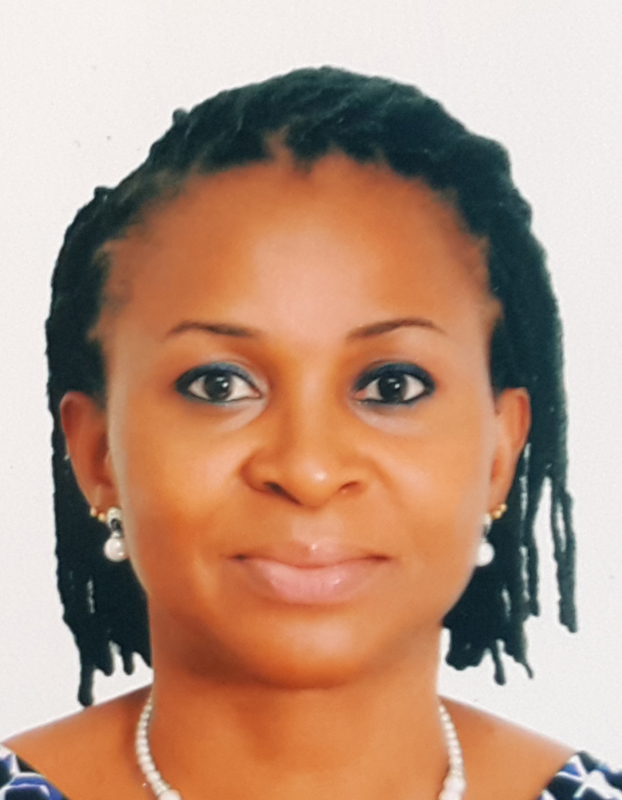
\includegraphics[width=5cm, height=6cm]{Olawale.jpg}}
\centerline{\caption{Photo of Ijeoma Olawale}}

\section{My Goals for CS 6000}
I am in my second semester as a PhD student in Security in the College of Engineering and Applied Sciences. I hope to learn about the research methods and publishing tools in Computer Science and how to effectively read, write and present research papers. With this knowledge gained, I hope to be able to develop my thesis proposal and write an acceptable thesis and research papers. 
My research interest is in the security of IoT and wearables; understanding the threats and attack surfaces that connected things like cars and healthcare gadgets face. As a security risk professional, I am concerned about the security and privacy issues that are prevalent with connected devices. These lack of security and privacy principles presents the potential for data integrity abuse, access control, authentication, authorization and non-repudiation issues. I hope that with the knowledge gained from CS 6000 I would be able to write a paper that can significantly contribute to the body of knowledge.
To spice up my life, I love taking road trips, going to the movies and attending live Christian concerts. I also love to volunteer because I believe that it is my little way of giving back and a chance to ‘pay it forward’. I volunteer as a Sunday school teacher at Crossroads Community Church, Parker CO and as a support crew with Winter Shelter Networks, Douglas county. I have volunteered as a DBA for Colorado Association of Black Professional Engineers and Scientists (CABPES) and I am exploring the opportunities to mentor and encourage middle and high school girls to take on careers in computer science and information security.



\end{document}
